% Conteúdo do capitulo
%1 - Descrição do desafio experimental para o ATLAS
%2 - Desafio de estabelecer o setup experimental
%3 - Desafio de melhorar o sensor LGAD
%4 - Desafio de aplicar para a medida de raios-x
%5 Considerações finais
\chapter{Desafios científicos e tecnológicos}

% 1 - Descrição do desafio experimental para o ATLAS
Como descrito anteriormente no texto, o desafio científico deste projeto é desenvolver um detector semicondutor - para a região de pseudo-rapidez frontal - capaz de melhorar a precisão da medida da luminosidade do feixe e a reconstrução de partículas no experimento ATLAS, para operar durante a fase de alta luminosidade do LHC ({\it High Luminosity LHC} (HL-LHC)) \cite{tdr}. 

Para superar esse desafio científico, este projeto irá trabalhar na pesquisa e desenvolvimento de um sistema de detecção frontal HGTD, cuja a técnica experimental é baseada na medida do tempo de voo das partículas com resolução capaz de medir intervalos de tempo menores do que 20-30ps \cite{tdr}, tornando dessa forma possível associar as partículas ao seu vértice de produção para colisões próton-próton no HL-LHC. Para realizar a construção do HGTD, os sensores do tipo LGAD serão adotados como base tecnológica, tendo em vista que eles apresentam excelentes características com respeito ao compromisso entre ganho e resolução temporal. 
% FASE 1
%2 - Desafio de estabelecer o setup experimental
A fase inicial do projeto terá como foco o desenvolvimento da metodologia experimental necessária para a caracterização dos sensores LGAD. Isso será feito através da implantação de três técnicas no laboratório de análises no HEPIC, com o objetivo de caracterizar os sensores LGAD em termos de sua corrente de fuga, ganho, uniformidade e resolução temporal. Nos parágrafos seguintes desta seção é descrito os passos que serão dados neste projeto para superar os desafios tecnológicos postos ao pesquisador responsável por esta proposta. 

Inicialmente será construída uma bancada de testes capaz de medir a corrente de fuga e a capacitância em função da voltagem aplicada ao sensor. A Fig. \ref{setup1} mostra um diagrama esquemático do arranjo experimental previsto para ser comissionado para este propósito.

\begin{figure}
    \centering
    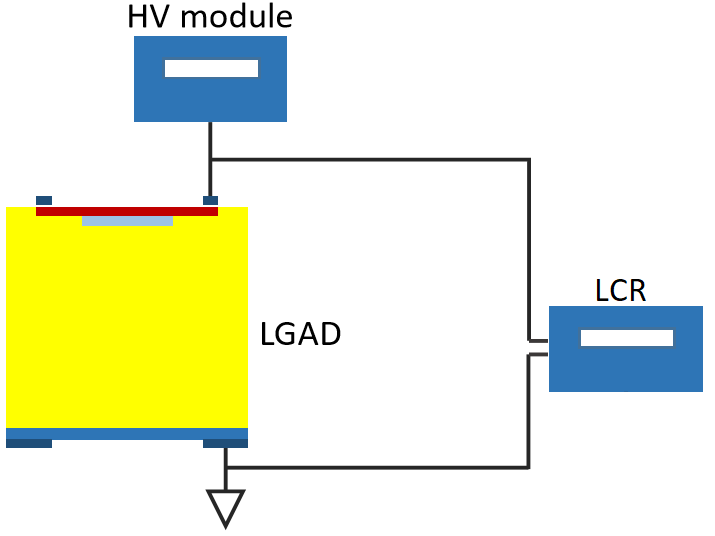
\includegraphics[width=10.0cm]{assets/iv_cv.png}
    \caption{Figura mostrando o diagrama para a medida de corrente e capacitância de um sensor LGAD.}
    \label{setup1}
\end{figure}

Em maiores detalhes, a montagem será composta por uma estação de prova onde os sensores serão acomodados durante os testes. Uma fonte de alta tensão com resolução para a medida de corrente será utilizada para aplicar a tensão e medir a corrente de fuga dos sensores - neste ponto cabe destacar que a utilização de pico amperímetros em conjunto com a fonte de tesão não é descartado. A medida da capacitância do LGAD será feita por intermédio de um Keysight LRC Analyser o qual permitirá medir a capacitância do sensor em função do bias aplicado. Por fim, todos esses equipamentos serão controlados por um programada de controle e aquisição dos dados o qual será produzido em ambiente LabView para monitorar as medidas e controlar sua qualidade.

Em seguida um setup dedicado será construído para medir o ganho dos sensores e a sua uniformidade. Nesta montagem será utilizado um laser vermelho de 660nm de pulso rápido - da ordem de pico segundos - o qual irá incidir na base do sensor produzindo elétrons de deriva devido à ionização do meio. Em seguida os elétrons serão coletados pelo campo elétrico presente na região de depleção do detector indo em direção à região de amplificação do dispositivo onde serão multiplicados. O sinal produzido neste processo será coletado no anodo e subsequentemente amplificado por intermédio de um amplificador externo sendo digitalizado em um osciloscópio. Finalmente, a carga coletada será medida através da integral da forma de onda fornecendo o valor do ganho do sensor. A uniformidade do sensor será medida com o mesmo princípio, por intermédio de uma varredura da posição de incidência do laser sobre a região sensível do sensor.

Por fim, para completar o conjunto de técnicas necessárias, a montagem de um sistema de medida precisa de tempo será feita para caracterizar os sensores em termos de sua resolução temporal. Para tanto serão necessários a utilização de uma fonte $\beta$ de $^{90}$Sr, um detector para atuar como trigger - o qual pode ser um detector Cherenkov de quartzo acoplado a um Silicon Photo Multiplier (SiPM) com resolução temporal de 10ps, ou outro sensor LGAD - e placas com eletrônica para acomodar o sensor e efetuar a leitura dos dados. Como mostra a Fig. \ref{setup2} neste arranjo o trigger será colocado atrás do LGAD, tornando possível medir apenas partículas com energia suficiente para atravessar o sensor. Neste sistema o trigger também sera lido por um osciloscópio. A resolução temporal será extraída da diferença entre a distribuição de tempo medida com o LGAD e o detector trigger.

\begin{figure}
    \centering
    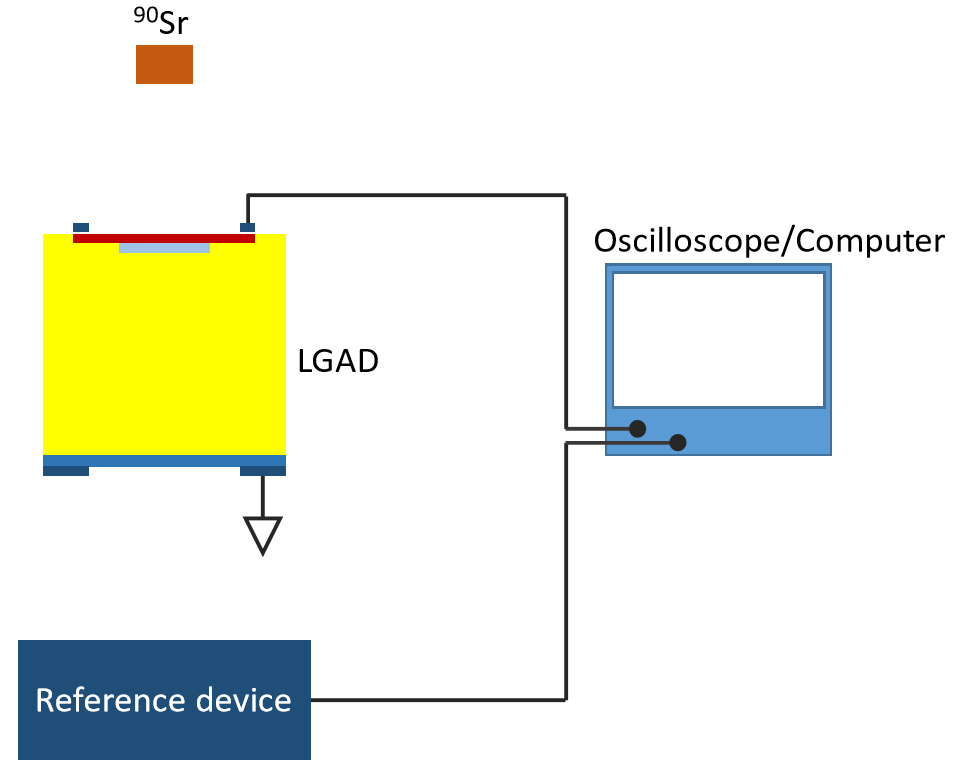
\includegraphics[width=10.0cm]{assets/time.png}
    \caption{Figura mostrando o diagrama para a medida da resolução temporal de um sensor LGAD.}
    \label{setup2}
\end{figure}

Com essas três técnicas estabelecidas será possível diagnosticar com precisão a performance dos sensores LGAD. Neste ponto, cabe ressaltar que o controle de temperatura é um componente importante para todas as técnicas de medida descritas anteriormente, e desse modo um controlador de temperatura será utilizado para estabilizar a temperatura do LGAD à -30$^{\circ}$ durante todas as medida que serão efetuadas, sendo essa a temperatura de operação nominal do HGTD \cite{tdr}.

À vista disso, cabe destacar que o grupo HEPIC possui competências adquiridas ao longo de anos de pesquisa dedicada a instrumentação que serão essenciais para o desenvolvimento deste projeto em sua fase inicial, tais como: design e confecção de placas eletrônicas para sensores, desenvolvimento de {\it Front End Electronics}, desenvolvimento de {\it Back End Electronics}, i.e firmware para aquisição de dados, e desenvolvimento de software para aquisição e análise de dados. Essas ferramentas aliadas à experiência do pesquisador responsável com o desenvolvimento de instrumentação científica \cite{tpcNIM,discharge_paper,THGEM} e com a colaboração com outros centros de pesquisa dentro da colaboração ATLAS e com o RD50 no CERN serão importantes para estabelecer de forma rápida as técnicas descritas anteriormente, garantindo a qualidade dos resultados obtidos e o sucesso dos investimentos feitos para pesquisa e desenvolvimento desses sensores. 

% FASE 2 - PROTOTIPAGEM DO LGAD
%3 - Desafio de melhorar o sensor LGAD
Uma vez consolidada os experimentos descritos acima para a caracterização dos sensores LGAD, o passo seguinte será continuar com o desenvolvimento do dispositivo, e com base nos dados coletados buscar discutir e optimizar os parâmetros do sensor com o objetivo de produzir novas gerações de LGAD com melhores características em termos de ganho, resolução temporal, uniformidade e resistência à radiação. 

Como dito anteriormente, o programa de pesquisa proposto neste projeto será em grande parte baseado na interação com a colaboração ATLAS, de modo que teremos acesso aos recentes avanços obtidos no desenvolvimento do LGAD, tais como a identificação de vulnerabilidades presentes na geometria do sensor e a inativação do material dopante devido ao dano radioativo, os quais serão também tópicos para investigação deste projeto.

Em maiores detalhes, com relação à geometria do LGAD, no atual estágio de desenvolvimento foi possível identificar fragilidades em seu design relacionados com regiões suscetíveis à ocorrência de descargas elétricas presentes nas bordas do sensor, onde o campo elétrico aplicado é mais elevado. Essa vulnerabilidade afeta a estabilidade elétrica do sensor, e essa questão será atacada no desenvolvimento dos próximos protótipos através de melhorias em seu {\it layout} as quais diminuam o campo elétrico em regiões críticas do sensor \cite{tdr}.  

Outro aspecto importante, o ganho em um detector LGAD é uma característica que depende diretamente do perfil da concentração de dopante presente na camada de multiplicação do sensor. Devido a presença dessa camada de amplificação o sensor torna-se mais complexo e mais suscetível à danos radioativos, levando em consideração que a inativação do dopante e a subsequente redução de sua concentração na camada de multiplicação pela incidência de radiação, provoca a redução do ganho e perdas na resolução em tempo. Para superar essa limitação tentativas preliminares demonstraram que a adição de outros materiais, tais como carbono, junto com o material dopante podem minimizar o impacto do dano radioativo tornando os sensores mais resistentes à radiação ionizante, entretanto com a contrapartida de diminuir a resolução em tempo \cite{tdr}. 

À vista disso, com a diminuição do ganho uma série de fatores surgem no escopo da pesquisa com o LGAD dentre eles o aumento da corrente consumida pelo dispositivo, o que por sua vez provoca o aumento na potência dissipada. Esse fator influencia o design de vários outros componentes que farão parte do detector para que seja possível dimensioná-los de forma adequada para comportar a carga de calor produzida pelo dispositivo. Estas questões  demonstram a grande importância de um estudo detalhado desses aspectos durante a fase de pesquisa e desenvolvimento do sensor. Até o momento os requisitos para a potência dissipada do dispositivo LGAD estão em aberto e serão abordados na produção dos próximos protótipos.

O cronograma de excussão do projeto para o desenvolvimento do LGAD da colaboração ATLAS se estenderá até o início 2021, afim de validar as possíveis modificações adotadas com relação ao {\it layout}, materiais empregados e diversos componentes e processos que serão empregados na produção dos dispositivos. Isso é essencial para assegurar que pontos importantes em relação ao sensor e sua integração sejam revisados e verificados de modo a atender as especificações requeridas pelo experimento ATLAS.

Como fica claro, o design final do LGAD encontra-se em seu estágio inicial de desenvolvimento, e desse modo inúmeras oportunidades para contribuição intelectual estão em aberto para serem exploradas na próxima fase da pesquisa e desenvolvimento que está para ser iniciada. De forma objetiva, o cronograma do projeto prevê a produção de dois lotes de dispositivos destinados à fabricação de protótipos para o início e segunda metade de 2020.%, onde são esperadas contribuições brasileiras para o desenvolvimento do dispositivo.

Por conseguinte, uma vez que todos os desafios técnicos forem superados, com o sensor e os fabricantes definidos, será iniciada a fase de fabricação dos dispositivos. Neste período a experiência adquirida durante a fase de desenvolvimento será fundamental para criar os procedimentos e protocolos requeridos com o objetivo de minimizar a probabilidade dos sensores apresentarem falhas durante a operação no experimento. Novamente, o grupo HEPIC e o pesquisador responsável participarão desta fase na criação das especificações para os sensores e os devidos protocolos para os testes.     

% FASE 3 -  
%4 - Desafio de aplicar para a medida de raios-x
Paralelamente à todas as atividades dedicadas ao desenvolvimento do LGAD em conjunto com a colaboração ATLAS, outros objetivos relacionados com a aplicação para a detecção de raios-X também serão somados a este projeto. Devido às excelentes características apresentadas, as quais incluem sua alta eficiência quântica para uma ampla faixa de comprimentos de onda, sensores semicondutores de diversos tipos são amplamente empregados na detecção de raios-X em experimentos que utilizam luz síncrotron. Com a vantagem de possuírem ganho intrínseco, dispositivos LGAD permitem a detecção de raios-X de baixa energia bem como a detecção de sinais produzidos por poucos fótons, sendo desta forma muito flexível. 

Com isso em mente, através da colaboração com o Laboratório de Sistemas Integráveis (LSI) da Escola Politécnica da USP será possível produzir sensores LGAD e modificar o seu perfil de dopagem de modo a produzir dispositivos com ganho adequado para operar no regime de avalanche proporcional optimizados para a detecção de raios-X. Por conseguinte, os dispositivos serão testados de forma rigorosa com os mesmos critérios aplicados aos sensores destinados para a colaboração ATLAS. Isso será um passo importante para estabelecer o domínio da tecnologia e a autossuficiência com respeito à produção desses dispositivos para aplicações no Brasil.

% CONSIDERACOES FINAIS

Por fim, fica evidente que esta proposta de projeto tem como objetivos estratégicos de curto prazo preparar os experimentos necessários para o desenvolvimento do LGAD no HEPIC, e por conseguinte colaborar com o experimento ATLAS na construção do HGTD. E para médio e longo prazo os objetivos de desenvolver dispositivos semicondutores para diversas aplicações científicas no âmbito nacional e internacional, e com isso consolidar a tecnologia para a fabricação de sensores semicondutores.

 %varios milestones estabelecidos

%Outro aspecto fundamental   

%Como descrito anteriormente, o ganho em um detector LGAD depende diretamente do perfil da concentração do dopante presente na camada de multiplicação do sensor. Dessa forma, o fator que mais contribui para o dano radioativo em sensores LGAD é a remoção e subsequente redução da concentração de dopante na camada de multiplicação o que por conseguinte provoca a redução do ganho e perdas na resolução em tempo. Com o R&D desenvolvido ate o momento, 

%preliminares demonstram que a adição de outros materiais, tais como carbono, junto com o material dopante podem minimizar o impacto do dano radioativo tornando os sensores mais resistentes à radiação ionizante, entretanto mais estudos devem ser conduzidos para compreender os fatores limitantes obtidos com a adição de outros materiais.


%incluindo a sua produção no Brasil. Vários pesquisadores que integram a equipe deste projeto vêm de outros grupos de pesquisa da USP, do IPEN, conferindo-lhe um forte carácter interdisciplinar, essencial no desenvolvimento de aplicações tanto em imagem de raios X, como na detecção de nêutrons.








